\chapter{Endormissement de tache sous priorité dynamique}
\minitoc
\section{modéle de tâches}
Le modèle utilisé ici est le modèle de tâche sporadique.

Soit $\taskset{} = \{\task{1},\task{2},...,\task{n}\}$ un ensemble de
tache, chaque tache $\task{i}$ est caracterisé par $\task{i} =
(\charge{i},\deadline{i},\period{i})$ et :

\begin{itemize}
\item $\task{i}$ est sporadique.
\item $\charge{i}$ est le pire temps d'execution de la t\^ache $i$
\item $\deadline{i}$ est l'écheance relative de la t\^ache $i$
\item $\period{i}$ est la periode de la t\^ache $i$
\item l'ensemble de tâches $\taskset{}$ est ordonnançable avec l'algorithme EarliestDeadlineFirst
\end{itemize}

\section{Limitation de nombre de preemption}

%\begin{center}
%\begin{algorithm}[H]
%\KwData{TaskSet de tâches sporadic $\taskset{}$}
%\KwResult{$Q(t)$}
%\Begin{
% Posons $\{t_{1},t_{2},...,t_{n}\}$ ensemble ordonné de $\{\deadline{i}+l\periode{i},\forall l \in N, 1 \leq i \leq n \}$ où $(t_{k} < t_{k+1},\forall k)$
% $Q(t_{1}) \leftarrow t_{1} - \sum_{\tache{i} \in \taskset{}} DBF(\tache{i},t_{1})$\;
% \For{$k \leftarrow 2,3...$}{
%	$Q(t_{k}) \leftarrow Min(Q(t_{k-1}),t_{k} - \sum_{\tache{i} \in \taskset{}} DBF(\tache{i},t_{k}))$\;
%	\If{$Q(t_{k}) < 0$}{
%	\textbf{return} faux\;
%	}
%	}
%	\textbf{return} vrai\;
% }
%\caption{Insertion Taches Endormissement Dans Un Mono-processeur}
%\end{algorithm}
%\end{center}

\section{Le cas monoprocesseur}
%\input{edfup.tex}

\begin{table}[!h]
\begin{center}
\begin{tabular}{|c|c|c|c|}
 \hline$\task{i}$ & $\charge{i}$ & $\deadline{i}$ & $\period{i}$ \\ 
 \hline 1 & 2 & 25 & 25 \\ 
 \hline 2 & 2 & 10 & 10 \\ 
 \hline 
 \end{tabular}
\end{center}
\caption{Ensemble de taches periodiques} \label{tab:exempleedfmp}
\end{table}

%\begin{figure}[h]
%\begin{center}
%\begin{RTGrid}[height=4cm,width=12cm,labelsize=8pt,numbersize=6]{3}{32}

%\multido{\n=0+25}{1}{
%\TaskArrDead{1}{\n}{25}}
%\TaskArrDead{1}{20}{10}

%\TaskExecution{1}{9}{10}
%\TaskExecution{1}{19}{20}
%\TaskExecution{1}{29}{30}

%\multido{\n=0+10}{3}{
%\TaskArrDead{2}{\n}{10}}
%\TaskArrDead{2}{15}{15}
%\TaskExecution{2}{0}{2}
%\TaskExecution{2}{10}{12}
%\TaskExecution{2}{20}{22}
%\TaskExecution{2}{30}{32}

%\multido{\n=0+10}{3}{
%\TaskArrDead{3}{\n}{10}}
%%\TaskArrDead{3}{25}{5}
%\TaskExecution{3}{2}{9}
%\TaskExecution{3}{12}{19}
%\TaskExecution{3}{22}{29}

%\end{RTGrid}
%\caption{Insertion de tache dans un monoprocesseur} \label{fig:exempleedfmp}
%\end{center}
%\end{figure}

\section{Le cas multiprocesseur}

%Réécris les algorithmes ici !! et pas dans un autre fichier en utilisant le package algorithmic !
%\input{edfmpl.tex}
%\input{edfmpg.tex}

\begin{table}[h]
\begin{center}
\begin{tabular}{|c|c|c|c|}
 \hline$\task{i}$ & $\charge{i}$ & $\deadline{i}$ & $\period{i}$ \\ 
 \hline1 & 2 & 10 & 10 \\ 
 \hline 2 & 2 & 15 & 21 \\ 
 \hline 
 \end{tabular}
\end{center}
\caption{Insertion locale de tâches d'endormissements dans un multiprocesseur} \label{tab:edfmp}
\end{table}
\section{insertion locale}
\begin{figure}[!h]
\begin{center}
\resizebox{15cm}{4cm}{
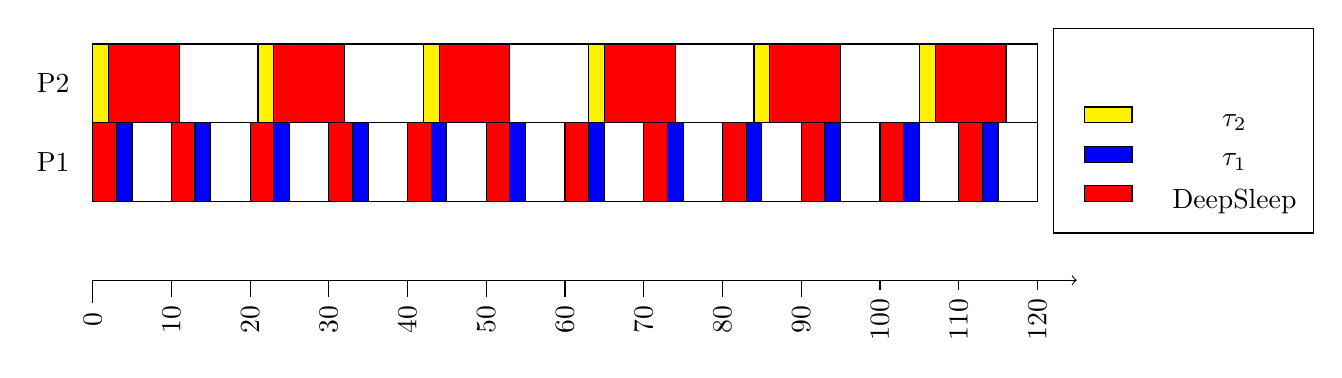
\begin{tikzpicture}
\node at (-0.5,0.5) {P1};
\node at (-0.5,1.5) {P2};
%P1
\draw[fill=white] (0.0,0) rectangle (12,1) ;

\draw[fill=red] (0.0,0) rectangle (0.3,1) ;
\draw[fill=blue] (0.3,0) rectangle (0.5,1) ;

\draw[fill=red] (1.0,0) rectangle (1.3,1) ;
\draw[fill=blue] (1.3,0) rectangle (1.5,1) ;

\draw[fill=red] (2.0,0) rectangle (2.3,1) ;
\draw[fill=blue] (2.3,0) rectangle (2.5,1) ;

\draw[fill=red] (3.0,0) rectangle (3.3,1) ;
\draw[fill=blue] (3.3,0) rectangle (3.5,1) ;

\draw[fill=red] (4.0,0) rectangle (4.3,1) ;
\draw[fill=blue] (4.3,0) rectangle (4.5,1) ;

\draw[fill=red] (5.0,0) rectangle (5.3,1) ;
\draw[fill=blue] (5.3,0) rectangle (5.5,1) ;

\draw[fill=red] (6.0,0) rectangle (6.3,1) ;
\draw[fill=blue] (6.3,0) rectangle (6.5,1) ;

\draw[fill=red] (7.0,0) rectangle (7.3,1) ;
\draw[fill=blue] (7.3,0) rectangle (7.5,1) ;

\draw[fill=red] (8.0,0) rectangle (8.3,1) ;
\draw[fill=blue] (8.3,0) rectangle (8.5,1) ;

\draw[fill=red] (9.0,0) rectangle (9.3,1) ;
\draw[fill=blue] (9.3,0) rectangle (9.5,1) ;

\draw[fill=red] (10.0,0) rectangle (10.3,1) ;
\draw[fill=blue] (10.3,0) rectangle (10.5,1) ;

\draw[fill=red] (11.0,0) rectangle (11.3,1) ;
\draw[fill=blue] (11.3,0) rectangle (11.5,1) ;
%P2
\draw[fill=white] (0.0,1) rectangle (12,2) ;

\draw[fill=yellow] (0.0,1) rectangle (0.2,2) ;
\draw[fill=red] (0.2,1) rectangle (1.1,2) ;

\draw[fill=yellow] (2.1,1) rectangle (2.2999999046325685,2) ;
\draw[fill=red] (2.2999999046325685,1) rectangle (3.1999999046325684,2) ;

\draw[fill=yellow] (4.2,1) rectangle (4.399999809265137,2) ;
\draw[fill=red] (4.399999809265137,1) rectangle (5.299999809265136,2) ;

\draw[fill=yellow] (6.2999997,1) rectangle (6.499999713897705,2) ;
\draw[fill=red] (6.499999713897705,1) rectangle (7.399999713897705,2) ;

\draw[fill=yellow] (8.4,1) rectangle (8.599999618530273,2) ;
\draw[fill=red] (8.599999618530273,1) rectangle (9.499999618530273,2) ;

\draw[fill=yellow] (10.5,1) rectangle (10.7,2) ;
\draw[fill=red] (10.7,1) rectangle (11.6,2) ;
%%%%%%%
\draw [->](0,-1) -- coordinate (x axis mid) (12.5,-1);
\draw (0,-1) -- (0,-1.5) node[fill=white,rotate=90] {0};
\draw (1,-1) -- (1,-1.5) node[fill=white,rotate=90] {10};
\draw (2,-1) -- (2,-1.5) node[fill=white,rotate=90] {20};
\draw (3,-1) -- (3,-1.5) node[fill=white,rotate=90] {30};
\draw (4,-1) -- (4,-1.5) node[fill=white,rotate=90] {40};
\draw (5,-1) -- (5,-1.5) node[fill=white,rotate=90] {50};
\draw (6,-1) -- (6,-1.5) node[fill=white,rotate=90] {60};
\draw (7,-1) -- (7,-1.5) node[fill=white,rotate=90] {70};
\draw (8,-1) -- (8,-1.5) node[fill=white,rotate=90] {80};
\draw (9,-1) -- (9,-1.5) node[fill=white,rotate=90] {90};
\draw (10,-1) -- (10,-1.5) node[fill=white,rotate=90] {100};
\draw (11,-1) -- (11,-1.5) node[fill=white,rotate=90] {110};
\draw (12,-1) -- (12,-1.5) node[fill=white,rotate=90] {120};

\draw[fill=white] (12.2,-0.4) rectangle (15.5,2.2) ;
\draw[fill=red] (12.6,0) rectangle (13.2,0.2) ;
\draw (14.5,0) -- (14.5,0) node[fill=white] {DeepSleep};
\draw[fill=blue] (12.6,0.5) rectangle (13.2,0.7) ;
\draw (14.5,0.5) -- (14.5,0.5) node[fill=white] {$\tau_1$};
\draw[fill=yellow] (12.6,1) rectangle (13.2,1.2) ;
\draw (14.5,1) -- (14.5,1) node[fill=white] {$\tau_2$};
\end{tikzpicture}}
\end{center}
\caption{Insertion globale de tâches d'endormissements dans un multiprocesseur} \label{fig:edfmpl}
\end{figure}
\section{insertion globale}
\begin{figure}[!h]
\begin{center}
\resizebox{15cm}{4cm}{
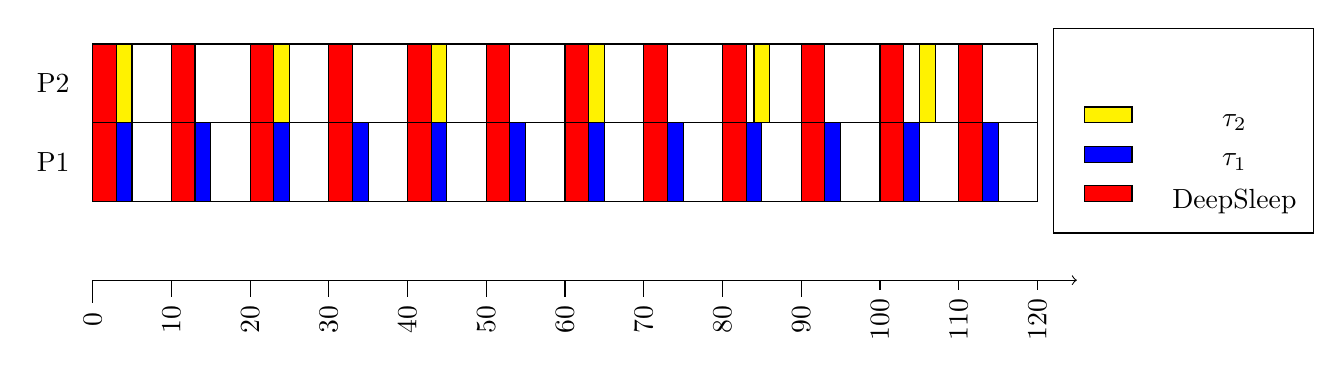
\begin{tikzpicture}
\node at (-0.5,0.5) {P1};
\node at (-0.5,1.5) {P2};
%P1
\draw[fill=white] (0.0,0) rectangle (12,1) ;

\draw[fill=red] (0.0,0) rectangle (0.3,1) ;
\draw[fill=blue] (0.3,0) rectangle (0.5,1) ;

\draw[fill=red] (1.0,0) rectangle (1.3,1) ;
\draw[fill=blue] (1.3,0) rectangle (1.5,1) ;

\draw[fill=red] (2.0,0) rectangle (2.3,1) ;
\draw[fill=blue] (2.3,0) rectangle (2.5,1) ;

\draw[fill=red] (3.0,0) rectangle (3.3,1) ;
\draw[fill=blue] (3.3,0) rectangle (3.5,1) ;

\draw[fill=red] (4.0,0) rectangle (4.3,1) ;
\draw[fill=blue] (4.3,0) rectangle (4.5,1) ;

\draw[fill=red] (5.0,0) rectangle (5.3,1) ;
\draw[fill=blue] (5.3,0) rectangle (5.5,1) ;

\draw[fill=red] (6.0,0) rectangle (6.3,1) ;
\draw[fill=blue] (6.3,0) rectangle (6.5,1) ;

\draw[fill=red] (7.0,0) rectangle (7.3,1) ;
\draw[fill=blue] (7.3,0) rectangle (7.5,1) ;

\draw[fill=red] (8.0,0) rectangle (8.3,1) ;
\draw[fill=blue] (8.3,0) rectangle (8.5,1) ;

\draw[fill=red] (9.0,0) rectangle (9.3,1) ;
\draw[fill=blue] (9.3,0) rectangle (9.5,1) ;

\draw[fill=red] (10.0,0) rectangle (10.3,1) ;
\draw[fill=blue] (10.3,0) rectangle (10.5,1) ;

\draw[fill=red] (11.0,0) rectangle (11.3,1) ;
\draw[fill=blue] (11.3,0) rectangle (11.5,1) ;
%P2
\draw[fill=white] (0.0,1) rectangle (12,2) ;

\draw[fill=red] (0.0,1) rectangle (0.3,2) ;
\draw[fill=red] (1.0,1) rectangle (1.3,2) ;
\draw[fill=red] (2.0,1) rectangle (2.3,2) ;
\draw[fill=red] (3.0,1) rectangle (3.3,2) ;
\draw[fill=red] (4.0,1) rectangle (4.3,2) ;
\draw[fill=red] (5.0,1) rectangle (5.3,2) ;
\draw[fill=red] (6.0,1) rectangle (6.3,2) ;
\draw[fill=red] (7.0,1) rectangle (7.3,2) ;
\draw[fill=red] (8.0,1) rectangle (8.3,2) ;
\draw[fill=red] (9.0,1) rectangle (9.3,2) ;
\draw[fill=red] (10.0,1) rectangle (10.3,2) ;
\draw[fill=red] (11.0,1) rectangle (11.3,2) ;

\draw[fill=yellow] (0.3,1) rectangle (0.5,2) ;
\draw[fill=yellow] (2.3,1) rectangle (2.5,2) ;
\draw[fill=yellow] (4.3,1) rectangle (4.5,2) ;
\draw[fill=yellow] (6.3,1) rectangle (6.5,2) ;
\draw[fill=yellow] (8.4,1) rectangle (8.6,2) ;
\draw[fill=yellow] (10.5,1) rectangle (10.7,2) ;
%%%%%%%
\draw [->](0,-1) -- coordinate (x axis mid) (12.5,-1);
\draw (0,-1) -- (0,-1.5) node[fill=white,rotate=90] {0};
\draw (1,-1) -- (1,-1.5) node[fill=white,rotate=90] {10};
\draw (2,-1) -- (2,-1.5) node[fill=white,rotate=90] {20};
\draw (3,-1) -- (3,-1.5) node[fill=white,rotate=90] {30};
\draw (4,-1) -- (4,-1.5) node[fill=white,rotate=90] {40};
\draw (5,-1) -- (5,-1.5) node[fill=white,rotate=90] {50};
\draw (6,-1) -- (6,-1.5) node[fill=white,rotate=90] {60};
\draw (7,-1) -- (7,-1.5) node[fill=white,rotate=90] {70};
\draw (8,-1) -- (8,-1.5) node[fill=white,rotate=90] {80};
\draw (9,-1) -- (9,-1.5) node[fill=white,rotate=90] {90};
\draw (10,-1) -- (10,-1.5) node[fill=white,rotate=90] {100};
\draw (11,-1) -- (11,-1.5) node[fill=white,rotate=90] {110};
\draw (12,-1) -- (12,-1.5) node[fill=white,rotate=90] {120};

\draw[fill=white] (12.2,-0.4) rectangle (15.5,2.2) ;
\draw[fill=red] (12.6,0) rectangle (13.2,0.2) ;
\draw (14.5,0) -- (14.5,0) node[fill=white] {DeepSleep};
\draw[fill=blue] (12.6,0.5) rectangle (13.2,0.7) ;
\draw (14.5,0.5) -- (14.5,0.5) node[fill=white] {$\tau_1$};
\draw[fill=yellow] (12.6,1) rectangle (13.2,1.2) ;
\draw (14.5,1) -- (14.5,1) node[fill=white] {$\tau_2$};
\end{tikzpicture}}
\end{center}
\caption{} \label{fig:edfmpg}
\end{figure}

